\chapter{Signals and Lanes \who{Grether, Thunig}}
\label{ch:signalslanes}
% ##################################################################################################################

\hfill \textbf{Author:} Dominik Grether, Theresa Thunig

\begin{center} 
\includegraphics[width=0.25\textwidth, angle=0]{figures/MATSimBook.png} \end{center}

% ##################################################################################################################

\section{Motivation}

%\mnote{Traffic Signal Control}
Traffic signals ensure security of travelers at junctions and regulate right of way. 
Furthermore, by assigning green times to the different approaches of a junction they are a determinant of the junctions performance. 
There are different strategies for traffic signal control: fixed-time traffic signal control for example repeats periodically the same schedule for signalization, whereas traffic-responsive signal control reacts dynamically on the prevailing traffic patterns to improve the performance of the junction or the system as a whole.   
Even if traffic %-responsive 
control improves the traffic conditions at a single junction, it might not result in benefits for the system as a whole. 
% As result of an improved traffic-responsive signal control at two single junctions, network wide changes in travel patterns can evolve}~\cite{Burghout2007HybridSimulationAdaptiveSignal}. 
\citet{Hu1997D2DFlowEvolutionReactiveSignalsDynasmart} argue that
second order or network effects should be taken into account when effects of signal control strategies are tested. Network effects include drivers' reactions not only in terms of route choice but also in terms of scheduling. 
Thus, traffic control and especially traffic-responsive signals need to obey some constraints. Otherwise, traffic may become unstable at the network level. 
%Thus, traffic-responsive signals can perform much worse than a fixed-time control in some situations~\citep{LaemmerHelbing2010SelfStabilizingSignalControlRealNet}. 
MATSim can capture most of these effects. 

This chapter reviews concepts, usage, and restrictions of the traffic signal control extension for MATSim. 
Before we will go into details a case study is reviewed to motivate traffic signal with MATSim. 

\subsection{Case Study}

The Cottbus scenario presented in Chapter~\ref{ch:scenarios:cottbus} is applied to illustrate the influence of traffic signal control. 
This section summarizes results published in~\citet{GretherBischoffNagel2011CottbusSylviaEventAbstract,Grether2014PhD}, readers interested in details are referred to these publications. 

%
The runs sequence of the base case is performed with three different signal control strategies:
%
In a first simulation sequence, all traffic signals are switched off. This can be used as a lower bound for results concerning signal control since it assumes that vehicles are able to traverse a crossing without any accident, i.e., they are able to drive ``through each other''. 
%
The next sequence uses the fixed-time setup. 
%
In the third, final, sequence, all traffic signals are controlled by a traffic-actuated stage length control. 
The control is based on the pretimed fixed-time schedules. 
The green times of the fixed-time schedules are reduced to a minimal green time of $5$/$10$ $sec.$. 
If at the end of this reduced green time vehicles are still approaching, the green time is extended up to a predefined maximum. 

\createfigure%
{Simulation Results}%
{Simulation Results}%
{\label{fig:results_histogram}}
{%
  \createsubfigure%
  {No vs.~fixed-time vs.~traffic-actuated signal control, commuter traffic, iteration 1000}%
	{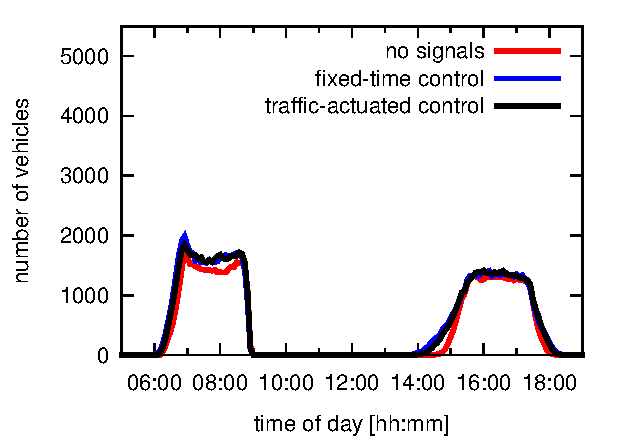
\includegraphics[width=0.48\linewidth]{extending/figures/signalslanes/leg_histogram_1292_1293_1291_it_1000.pdf}}
  {\label{fig:commuter_traffic}}%
  \createsubfigure%
	{Average travel time for unexpected event traffic, iteration 1000}
	{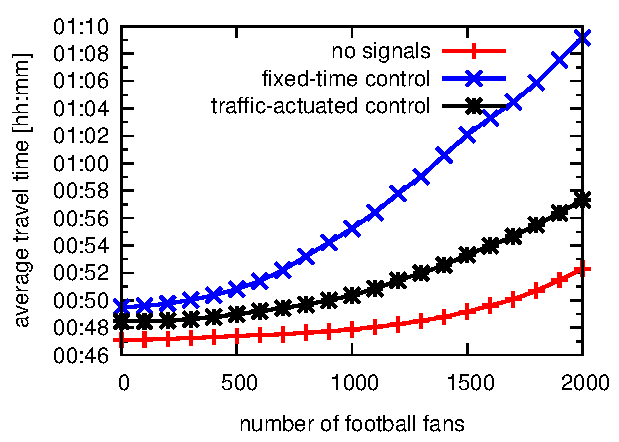
\includegraphics[width=0.48\linewidth]{extending/figures/signalslanes/average_travel_time_1220_1222.pdf}}
	{\label{fig:unexpected_event}}
}%
{Source:~\citet{Grether2014PhD}}

Simulation results for iteration 1000 of the Cottbus commuter scenario are depicted in
Fig.~\ref{fig:commuter_traffic}. 
The number of vehicles simultaneousely on the road is plotted over the time-of-day. 
%Due to the nature of a commuter scenario characterized by a steady
%demand over a certain time horizon 
The results are quite similar for all signal control strategies. 
The differences are small because of the lack of heavy congestion in the Cottbus scenario. 

A change of signal control has more effect if some unexpected traffic occurs in the network. 
It is assumed that the local soccer club ``FC Energie Cottbus'' has a derby that takes place on a normal weekday, thus interfering with the regular commuter traffic. 
In the last iteration of the run sequences, in addition to the commuters $0$ to $2000$ vehicles drive to the soccer stadium of Cottbus during the evening peak. 
It is assumed that 25 \% of these fans come from Cottbus,
while the other 75 \% come from the ``Spree-Nei{\ss}e'' area around Cottbus, and that all fans start their trips between 17:00 and 18:00. 

Fig.~\ref{fig:unexpected_event} plots the number of soccer fans on
the x-axis, and the average travel time of all travelers on the
y-axis. Without any additional vehicles,
the traffic-actuated signal control leads to a gain of
approx.~$1 \, min$ per traveler.
The more additional traffic is approaching the stadium, the more the traffic-actuated control saves travel time. In the case where 2000 additional vehicles are on the road, travel time savings reach ca.~$15\, min$~per traveler. 

Summarizing: In slightly jammed commuter scenarios, simulation results with a change in traffic signal control that leads to heavily decreased overall travel time have not been simulated with MATSim, yet. 
Looking at different objectives with more fine grained analysis tools can reveal network wide effects~\citep[e.g.~see the analysis using macroscopic fundamental diagrams, pp.114]{Grether2014PhD}, but this is work in progress.  
More heavily jammed scenarios can increase the overall traffic impact of a change in traffic signal control. The case study show significant effects of traffic-responsive signal control, if something unexpected happens and travelers do not react.  

\subsection{Overview}

The presented case study highlights some already researched aspects of MATSim simulations with traffic signals. 
Sec.~\ref{sec:signals_traffic_signal_control} provides some traffic signal control vocabulary and backgrounds.  
MATSim is not the tool of choice for all questions concerning traffic signal control. 
The codebase, however, can also help to simulate other use cases, e.g.~evacuation or air transport scenarios. 
The remaining chapter provides deeper insight.  
MATSim's open source nature provides hooks and interfaces for extension. 
But you should consider the amount of work required to get things done in respect to the current state of development and your project planning. 
If you need highly detailed traffic flow models or a high detail network representation, you should consider other tools. 
Sec.~\ref{sec:signals_network_traffic_flow} goes into details of network and traffic flow modeling. 
If your requirements are met, Sec.~\ref{sec:signals_iterations_learning} considers iterations and learning. 
When it comes to agent based learning, MATSim is very fast -- the presented case study requires on average~$17$ seconds computation time per iteration -- for scoring, replanning, and output. One complete run sequence ($1000$ iterations, single core mobility simulation, multi core replanning) was simulated in $9 \, h$ and $12 \, min$. 
The speed of simulation leaves room for exploration of network wide behavioral reactions on changes of traffic signal control. 
Furthermore, the resource efficient simulation enables the joint simulation of several policies. 
%Before you present your results to public, you should consider certain aspects concerning the  evaluation and interpretation of simulation results, Sec.~\ref{sec:signals_evaluation}. 
When you decide to go the MATSim way, consider Sec.~\ref{sec:signals_traffic_signals_in_matsim} for some MATSim specific hints and Sec.~\ref{sec:signals_conclusion} for some last checks. 

%Thus, it is well worth to consider a extension for the simulation of traffic-responsive signal control. Further, the impacts of recently developed optimization models for fixed-time control can be tested~\citep{KoehlerStrehler2010SignalDemandOptimization}. 


\section{Traffic Signal Control}
\label{sec:signals_traffic_signal_control}



%\mnote{Optimization of Fixed-Time Control} 
Fixed-time traffic signal control periodically assigns a well-defined green-split for each approach of a junction. 
Traditionally, for optimization of fixed-time signals different regimes of equilibrium traffic flow are determined for several periods of time, e.g., weekday morning, midday, evening and night plus a separate estimate for weekends.   
These traffic flows serve as input for optimization~\citep[e.g.~][]{Webster1961SignalSettings,Allsop1972SignalizedJunctionCapacity,Allsop1991SignalsStageBased,Robertson1969Transyt}.  

%\mnote{Traffic-Actuated Control}
With upcoming availability of sensors and computer technology these optimizations provided the basis for traffic-actuated signal control strategies. 
Based on detector input fixed-time signal parameters as green times, cycle, and offsets are adjusted to current traffic situations on the fly. 
Some actuated approaches use logical operators and functions to adjust signal timings~\citep{Friedrich2002VerkehrsadaptiveLSASteuerung}. More advanced methods as, e.g., SCOOT~\citep{HuntEtc1981SCOOT,RobertsonBretherton1991ScootMethod,BrethertonBodgerBaber2004ScootFuture}, MOTION~\citep{BielefeldtBusch1994MOTION,BuschKruse2001MotionSITRAFFIC,BrilonEtAl2009MotionMuenster}, or BALANCE~\citep{GEVAS2011Balance,BraunEtAl2009TravolutionLSA2CarCommunication} use macro- and mesoscopic traffic models to predict effects of adjustments of signal timings for a certain time horizon.  
%

%\mnote{Adaptive Control}
Recent approaches for traffic signal control no longer need a fixed-time control that is adjusted. 
Instead, the signal program is build completely on-the-fly based on sensor information.  
%
These methods originate from different areas of science. 
One finds rather conceptual studies and methods that can and are used in practice. 
%TUC
An example for the latter is TUC (traffic-responsive urban control)~\citep{DiakakiPapageorgiouAboudolas2002MultivariableRegulatorTUC,DiakakiEtAl2003ExtensionsTUC,KrausEtAl2010CostEffectiveSignalsTUC,AboudolasEtAl2010RollingHorizonTUC,KouvelasEtAl2011HybridStrategyTUC} a control theoretic strategy that uses a linear-quadratic regulator approach to control green splits based on a store-and-forward model of urban traffic. 
Due its polynomial complexity TUC can be used in real time monitoring the whole transport network. 
Optional extensions to TUC provide cycle time adjustments, offset optimization, and public transit priority.   
Also practice ready is the approach proposed by~\citet{Laemmer2007PhD,LaemmerHelbing2008SelfControlTrafficLights,LaemmerHelbing2010SelfStabilizingSignalControlRealNet}. 
In undersaturated traffic conditions a priority based optimization of scheduling minimizes local waiting times. 
A second module stabilizes the optimization when traffic density increases. 
Green waves are established locally by a prediction model for future arrivals. 
%
Rather conceptual is the approach proposed by~\citet{CoolsEtAl2007SelfOrgSignalsSimulation,GershensonRosenblueth2009SelfOrgSignalsWithCA} that looks at traffic as a self-organizing system~\citep{ElmenreichEtAl2009SelfOrganizingSystemsSurvey}. 
Traffic signals can be controlled by a set of simple rules, coordination evolves from the interaction between cars and signals. 
Sensor information, however, can be erroneous as some detectors may not work at all or provide incorrect data. 
If sensor data is erroneous, quality of an adaptive signal control may drop. 
This problem is addressed by~\citet{OertelWagner2011DelayTimeActuatedSignals}. 
Advanced traffic detection technologies as, e.g., GPS data or video processing, measure the delay imposed to individual vehicles approaching a signal. 
When the delay is below a certain threshold a queue clearing policy terminates a green phase.  
Noteworthy, in simulation studies, the signal control outperforms other approaches when only a part of the individual vehicle delays can be detected. 

%\mnote{Agents}
Intelligent agents~\citep{RusselNorvig2010ArtificialIntelligence} can be used to control traffic signals of one or several junctions~\citep{Bazzan2005signalAgents}. 
Reinforcement learning techniques enable the agents to control traffic flows~\citep{Bazzan2005signalAgents,BazzanOliveiraSilva2010LearningTrafficSignals,Bazzan2009ReinforcementLearningPrint}.  
Besides agent-based approaches, signalized junctions can be controlled by other techniques as autonomic and organic computing~\citep{Prothmann2010OrganicSignalControl}. 

\begin{itemize}
	\item MATSim provides support for all kinds of strategies: Fixed-time, traffic-actuated, adaptive, network wide, organic and so on..
	\item Fixed-time control as basic implementation
	\item The rest, whatever is meaningful for you to implement
\end{itemize}

\section{Network Representation \& Traffic Flow}
\label{sec:signals_network_traffic_flow}

\createfigure%
{Caption in List of Figures}%
{Influence of traffic signals on traffic flow and spill-back can be modeled by a queue model, if the layout of turn pockets is considered.}
{\label{fig:lanes_representation}}%
{%
  \createsubfigure%
	{Single queue, spill-back is not captured correctly}%
	{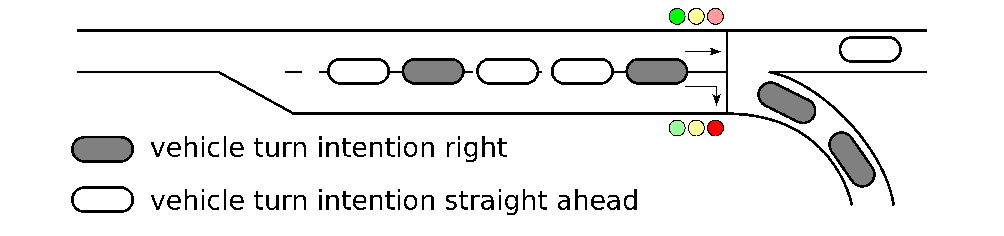
\includegraphics[width=0.48\textwidth]{extending/figures/signalslanes/single_queue_model_inkscape.pdf}}%
	{\label{fig:lanes_representation_single_queue}}%
  \createsubfigure%
	{Multiple queues, spill-back is captured correctly}%
	{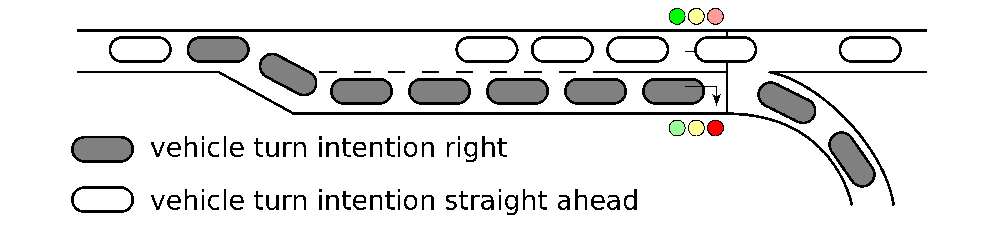
\includegraphics[width=0.48\textwidth]{extending/figures/signalslanes/multiple_queue_model_inkscape.pdf}}%
	{\label{fig:lanes_representation_multiple_queue}}%
}%
{info about source (optional)}

Waiting queues for distinct turning movements, including their spatial extension are modeled explicitly. 
For that reason, in case of spill-back mutual blocking effects between several turning directions are captured.
This is important if traffic signals are simulated microscopically, see Fig.~\ref{fig:lanes_representation}: If a single queue is used (Fig.~\ref{fig:lanes_representation_single_queue}), the first vehicle blocks all other vehicles upstream. 
This can capture reality if the approach has only one lane for all turning moves but does not hold in all cases. 
In the case, however, that the approach has several lanes for signalized turning-moves, a single queue model distorts the effects of signalization. 
In contrast, Fig.~\ref{fig:lanes_representation_multiple_queue} shows the modeling approach from~\cite{CremerLandenfeld1998MesoTrafficSignalModel}. Vehicles with distinct turn intentions do not block each other until the available space for queueing on the lane is used completely.


Fig.~\ref{fig:real_road_layout} illustrates a typical layout of a real-world road segment with several turning lanes at its end. 
The layout of the corresponding graph is shown in Fig.~\ref{fig:model_link_layout}. 
If each edge is represented by a link of the Gawron model spill-back effects between turning lanes are captured. 
\createfigure%
{Caption in List of Figures}%
{Transition from a real road segment to a graph layout}
{\label{fig:combined_model}}
{%
  \createsubfigure%
	{Typical real road layout}
	{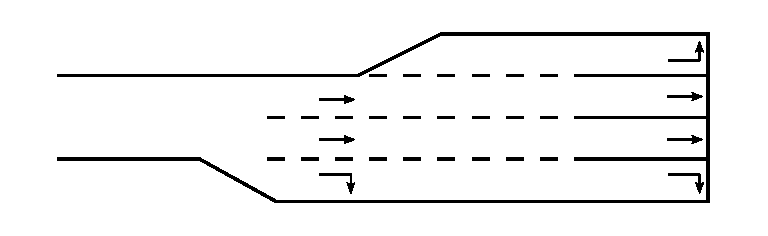
\includegraphics[width=0.475\linewidth]{extending/figures/signalslanes/real_road_layout.pdf}}
	{\label{fig:real_road_layout}}
  \createsubfigure%
	{Part of the graph required to model the road layout}
	{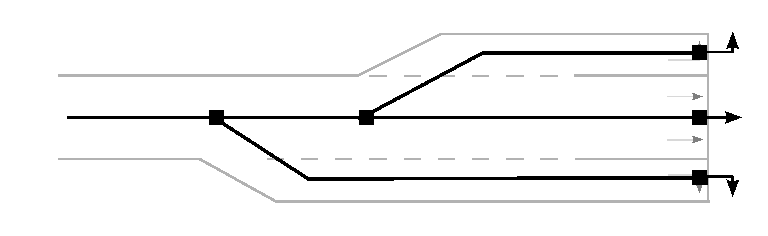
\includegraphics[width=0.475\textwidth]{extending/figures/signalslanes/link_lanes_layout}}
	{\label{fig:model_link_layout}}
}%
{info about source (optional)}



\subsection{Traffic Flow Modeling}

\begin{itemize}
	\item traffic flow linear to green time
	\item see also LaemmerPhd
\end{itemize}

\subsection{Findings}

\begin{itemize}
	\item Can you modify your network?
	\item Do you want to have a comparison between network with and without lanes?
\end{itemize}




\section{Iterations \& Learning}
\label{sec:signals_iterations_learning}


%\mnote{Equilibrium?}
Using Wardrop equilibrium assumptions and continuous link costs,~\citet{Smith1979ExistenceUniquenessStabilityEquilibria} shows the existence of a unique and stable static traffic equilibrium. 
This provides the underlying theory to prove, that traffic signal control influences route choice~\citep{Smith1979TrafficControlRouteChoice}. 
The existence of a dynamic traffic equilibrium is studied by~\citet{Smith1993ModelDynamicUE}. 
\citet{SmithVanVuren1993TrafficEquilibriumResponsiveControl} propose an optimization algorithm for dynamic assignments that takes traffic-responsive signal control into account.  
The dynamic formulations do not consider the physical extent of queues, they are built up on point-queues. 

%\mnote{Combined Problem}
The combined modeling of the traffic signal control and traffic assignment is subject of several other research lines. 
\citet{Meneguzzer1997ModelReviewTrafficAssignmentSignalControl} reviews their initial roots and defines the {\bf combined traffic assignment and control problem} (CTAC) as finding a tuple $(f^{*}, g^{*})$ of traffic flows $f$ and signal settings $g$ under policy $P$ that fulfills  
\[
f^{*} = f^{e}[g^{P}(f^{*})] \mbox{  or  equivalently } g^{*} = g^{P}[f^{e}(g^{*})]
\]
where $f^{e}$ is a function mapping signal settings to equilibrium traffic flows and $g^{P}$ a function mapping from traffic flows to signal settings under policy $P$.  
Nicely, the formulation shows the mutual interaction of traffic patterns and signal settings. 
A similar problem formulation is given by~\citet{CascettaGalloMontella2006SignalsWithStochAssignment}, studying the difference between global and local signal optimization. 
The time horizon, on that these interactions take place, is not captured by the formulations. 

%\mnote{Game theory}
Solution techniques for game theoretical models and mathematical programs with equilibrium constraints are similar, especially for bi-level, Stackelberg games~\citep{Hollander2006NonCooperativeGamesTransport}. 
Game theory provides techniques and terminology to describe the social dilemma of self-interest vs cooperation between distinct players. 
For transportation systems game theory provides ''a framework for modeling interactions between groups of decision makers when individual actions jointly determine the outcome''\citep{Fisk1984GameTheoryTransportationSystems}. 
The definition of a ``leader'' is required to model the decisions of a transport authority and the response of traffic participants as Stackelberg game. 
%
Mathematical programs also comprise such assumptions but they often are intrinsic to the model and not discussed. 
%
A broad review of games used to model and analyze transport systems was undertaken by~\citet{Hollander2006NonCooperativeGamesTransport}. 
Classical game theory is static an explicit representation of time is missing. 
In most cases traffic flows are modeled statically. 

%\mnote{Space \& Time}
Under the assumption that interactions between travelers and traffic signals over space and time have nicely behaved mathematical properties~\citet{Hu1997D2DFlowEvolutionReactiveSignalsDynasmart} use DYNASMART\footnote{see~\url{http://mctrans.ce.ufl.edu/featured/dynasmart/}, last access 17.05.2013} for simulation. 
Traffic signal control and travelers' reactions are studied in a day-to-day and real-time context. 
Traffic-responsive control may improve throughput of a traffic network. 
The peak load of the network stays equal. 
The travelers use the improvements to reduce schedule delay~\citep{Hu1997D2DFlowEvolutionReactiveSignalsDynasmart}. 
\citet{Burghout2007HybridSimulationAdaptiveSignal} build a hybrid simulation by a combination of a microscopic and a mesoscopic traffic simulation model. 
The replacement of a fixed-time control by a traffic-actuated signal control at two junctions changes the travel patterns in the city-wide network. 

%\mnote{Dynamics \& Game Theory}
Game-theoretic formulations for the dynamic interactions between traffic control and traffic assignment are given by~\citet{ChenBenAkiva1998GameDynamicTrafficControl}. 
Depending on the type of game used to model the problem, the quality of the solution with respect to the objective function differs.  
The solution of a monopoly game represents the optimal solution that can be used as benchmark. 
A Stackelberg equilibrium is superior to the Cournot-Nash equilibrium as user reactions are anticipated~\citep{ChenBenAkiva1998GameDynamicTrafficControl}\footnote{
%
The Cournot-Nash equilibrium is defined as follows: 
``In a noncooperative game between a traffic authority and highway
users, a combination of strategies $(g^*, h^*)$ is a Cournot(-Nash) equilibrium
$\Leftrightarrow$ control plan $g^*$ is the traffic authority's best
response to flow $h^*$, and flow $h^*$ is the users' 
%\kai{paper sagt user's (sing.), aber m.E.\ sollte es users' (plural) sein??} 
best response to control plan $g^*$'' \citep[from][]{ChenBenAkiva1998GameDynamicTrafficControl}.
%
\\
%
The Stackelberg equilibrium improves over the Cournot equilibrium in
that the traffic control authority anticipates the users' reactions:
``$\ldots$, a strategy combination $(g^*,h^*)$ is a Stackelberg
equilibrium $\Leftrightarrow$ it solves the following bilevel
programming problem: $\min_g Z[g,h^*(g)]$ such that flow $h^*(g)$ is
the users' best response'', where $Z$ is the traffic authority's
objective function \citep[after][]{ChenBenAkiva1998GameDynamicTrafficControl}.
%
\\
%
In the system optimum ($=$ monopoly game), the traffic authority also
controls the user flows; the optimization problem becomes: $\min_{g,h}
Z[g,h]$.
%
}.

Mutual effects between road users and two different road authorities responsible for traffic signal control are investigate by~\citet{VanZuylenTaale2004UrbanRingRoads} in an analytic, static setup, and by simulation.  
In a Stackelberg game, one of the road authorities takes the role of the leader. 
The other authority and the road users react to the decisions of the leader. 
Results for the analytical solution differ according to the leader of the Stackelberg game.  
Same holds for the presented dynamic simulation studies. 
Best results, however, are reported when both authorities cooperate and anticipate the road users' reaction on the traffic signal control. 
%\mnote{Physical Queues}
Noteworthy, the simulation model takes into account physical queue length~\citep{TaaleVanZuylen2003AnticipatoryTrafficControl} and is refined in further works to capture spill-back effects between links of the transport network~\citep{Taale2008Phd}. 
In a more general context, the importance of modeling physical queues for dynamic assignment is emphasized by~\citet{DaganzoAssign-w-queues}.  
The temporary limited effect of queue spill-back in conjunction with a dynamic assignment may lead to situations where the equilibrium is no longer unique.  

%\tododg{look at : I think so, should check the other Cascetta references in there? s.o. bzw discussion }

%\mnote{Agents \& Evolutionary Games}
In general, agent- and mechanism-design both can benefit from use of game theory~\citep[][pp.~666]{RusselNorvig2010ArtificialIntelligence}. 
Most mentioned approaches use classical game theory and the Nash equilibrium assumptions, i.e., the impact of a strategy is assumed to be fully known by all players. 
The approaches modeling interactions between traffic control and travelers that take time-scales into account use iterative solution techniques. 
Traffic assignment is solved iteratively and at least partly via simulation. 
\citet{Hu1997D2DFlowEvolutionReactiveSignalsDynasmart} report amongst other as result the number of ``days''~\footnote{one iteration represents one day} until convergence as measure of effectiveness. 
To describe the dynamic interactions between players, also evolutionary game theory can be used~\citep[e.g.~][]{HofbSigmBook}. 
While classical game theory looks for equilibrium solutions, evolutionary game theory searches strategies that are evolutionarily stable \citep[p.~348]{Bazzan2009ReinforcementLearningPrint}. 
Thus, use of evolutionary game theory helps when learning processes are included in the model. 
E.g., the agents that learn to control signalized junctions proposed in~\citet{Bazzan2005signalAgents} are useful if they are able to learn quickly but useless if learning takes infinite time. 
Evolution seems plausible on both sides of the game -- \citet[e.g.~][]{BazzanEtc2008co-evolution-of-tr-lights-lncs} signalized junctions \emph{and} car drivers are modeled as learning agents. 

\begin{itemize}
	\item Who is learning what? 
	\item No best way found
	\item Document what you have done
\end{itemize}


\section{Traffic Signals in MATSim}
\label{sec:signals_traffic_signals_in_matsim}

\begin{itemize}
	\item How to adapt the config file?
	\item Which additional files are needed?
	\item Refer to the user guide.
\end{itemize}


\section{Conclusion}
\label{sec:signals_conclusion}

\subsection{Evaluation \& Interpretation}

\begin{itemize}
	\item Evaluation criteria manifold
	\item BUT: Matsim model only simulates a part of it
	\item Do Not over-interpret results, implement and interpret everything in respect to other simulation steps, document what you have done
\end{itemize}


\subsection{Conclusion, why -- again}

\begin{itemize}
	\item After reading a lot of constraints, why do not use another tool?
	\item Network wide effects
	\item Simulation results consistent with model's implementation 
	\item Economic evaluation
	\item Diversity 
	\item Go!
\end{itemize}

\section{Automatically Generated Module Information}
Module in the config: 
\begin{itemize}
	\item \lstinline|signalsystems|
\end{itemize}

Package:
\begin{itemize}
	\item \lstinline|org.matsim.signalsystems|
\end{itemize}

http://matsim.org/node/732

Literature: \citet[][]{GretherEtAl_ABMTRANS_2012, Grether_PhDThesis_2014, Neumann_MastersThesis_2008}
Auch Miss Ou-Paper ansehen: Optimierung von Lichtsignalen

\citet[][p.?]{BalmerEtAl_ResRep_bdktzrh_2009}


Information about signal light timing are available for the city of Zurich  \citep{STAPOZH-DAV_unpub_gtZH_2008} (\ref{ptl:zhCity}). Modeling of traffic lights was implemented for the project \emph{Westumfahrung} trough reducing the available link capacity. However, the used \emph{mobsim} (DEQSim) is deprecated (see Section \ref{sec:deqsim}).

Research and implementation efforts are undertaken to include individual traffic lights in other \emph{mobsims} (see e.g., (\ref{tl:docu}) and \citet[][]{Neumann_MastersThesis_2008}).

% -------------------------------------------

Lanes:

The lanes package has been implemented in conjunction with signal systems. Lanes are enabled in the \lstinline|scenario| configuration file section. The lanes package (\lstinline| org.matsim.lanes|) provides readers, where the class \lstinline|ModelLane| serves as the interface between the lane functionality and the mobility simulation. The lane definitions file needs to be specified in the \lstinline|network| configuration file section.

% ##################################################################################################################
